\chapter{Thermodynamics of reacting ideal-gas mixtures}
\label{ch:thermo}

Thermodynamics answers two questions: \emph{how much energy} is released when a mixture reacts,
and \emph{where it ends up} if left alone for long enough. It says nothing about how fast; that is
kinetics (\chapref{ch:kinetics}).

\section{System, state and properties}

A \textbf{system} is the piece of matter we look at. Its \textbf{state} is fully fixed by a small
number of \textbf{state variables}. For a gas mixture of $K$ species, the \emph{state postulate} says
that two thermodynamic variables plus the composition are enough:
\begin{equation}
  \text{state} = \big(T,\;p\ \text{(or }\rho),\;\text{composition }Y_1,\dots,Y_K\big).
\end{equation}
Everything else ($h$, $s$, $c_p$, viscosity, reaction rates\dots) is a function of these. In
Cantera this is literally the statement \code{gas.TPY = T, p, Y}: after it, every property is
available.

\textbf{Extensive} properties scale with the amount of matter (volume $V$, enthalpy $H$);
\textbf{intensive} ones do not ($T$, $p$). Dividing an extensive property by mass gives a
\emph{specific} property (lower case, per kg: $h=H/m$); dividing by moles gives a \emph{molar}
property (with a hat or bar, per kmol: $\hat h = H/n$).

\section{The ideal gas}
\label{sec:idealgas}

\begin{derivation}[ideal gas law from molecules hitting a wall]
Consider $N$ molecules of mass $m$ in a box of volume $V$. A molecule with velocity component
$c_x$ that hits the wall at $x=L$ bounces back with $-c_x$: momentum change $2mc_x$. It returns
after time $2L/c_x$, so its average force on the wall is $2mc_x/(2L/c_x)=mc_x^2/L$. Summing over
all molecules and dividing by area $A$:
\[
p = \frac{\sum m c_x^2}{L A} = \frac{N m\overline{c_x^2}}{V}=\frac{N m\overline{c^2}}{3V},
\]
because $\overline{c^2}=\overline{c_x^2}+\overline{c_y^2}+\overline{c_z^2}=3\overline{c_x^2}$ by symmetry.
Temperature is \emph{defined} microscopically through the mean kinetic energy,
$\tfrac12 m\overline{c^2}=\tfrac32 k_B T$, so $pV=Nk_BT$. With $n=N/N_A$ moles and
$\Ru=N_Ak_B$:
\begin{equation}
  pV=n\Ru T\qquad\Longleftrightarrow\qquad p=\rho\frac{\Ru}{W}T,
  \label{eq:idealgas}
\end{equation}
where $W$ is the molar mass [kg/kmol] and $\rho=nW/V$.
\end{derivation}
\begin{symbols}
$N$ & number of molecules in the box & \nodim\\
$m$ & mass of one molecule & \si{\kilo\gram}\\
$V$, $L$, $A$ & box volume, box length, wall area & \si{\metre\cubed}, \si{\metre}, \si{\metre\squared}\\
$c_x$, $c$ & molecular velocity component normal to the wall, molecular speed & \si{\metre\per\second}\\
$\overline{c^2}$ & mean of the squared molecular speed & \si{\metre\squared\per\second\squared}\\
$p$ & pressure (force per unit wall area) & \si{\pascal}\\
$k_B$ & Boltzmann constant, $1.380649\times10^{-23}$ & \si{\joule\per\kelvin}\\
$T$ & temperature & \si{\kelvin}\\
$n$ & amount of substance & \si{\kilo\mole}\\
$N_A$ & Avogadro's number, $6.022\times10^{26}$ & \si{\per\kilo\mole}\\
$\Ru=N_Ak_B$ & universal gas constant & 8314.46 \si{\joule\per\kilo\mole\per\kelvin}\\
$W$ & molar mass & \si{\kilo\gram\per\kilo\mole}\\
$\rho$ & density & \si{\kilo\gram\per\metre\cubed}\\
\end{symbols}

\begin{intuition}
Pressure is the momentum flux of molecules hammering the wall; temperature is how hard each one
hits. ``Ideal'' means the molecules do not attract each other and take up no volume. At flame
conditions (high $T$, moderate $p$) this is an excellent approximation. Note: the typical
molecular speed $\sqrt{3k_BT/m}$ is $\sim\SI{500}{\metre\per\second}$ for \ce{N_2} at room
temperature and $\sim\SI{1900}{\metre\per\second}$ for \ce{H_2}. Light molecules are fast,
which is why hydrogen diffuses so quickly (\chapref{ch:transport}).
\end{intuition}

\section{Describing a mixture}
\label{sec:composition}

Let species $k$ have $n_k$ kmol, mass $m_k=n_kW_k$, in a volume $V$. Three ways to describe the
composition:
\begin{align}
  \text{mole fraction}\quad & X_k=\frac{n_k}{\sum_j n_j}, &&\textstyle\sum_k X_k=1,\\
  \text{mass fraction}\quad & Y_k=\frac{m_k}{\sum_j m_j}, &&\textstyle\sum_k Y_k=1,\\
  \text{molar concentration}\quad & C_k=[X_k]=\frac{n_k}{V}\ \ [\si{\kilo\mole\per\metre\cubed}].
\end{align}

\begin{derivation}[conversions]
The \textbf{mean molar mass} is total mass over total moles:
\begin{equation}
  W=\frac{\sum_j n_jW_j}{\sum_j n_j}=\sum_j X_jW_j
  \qquad\text{and equivalently}\qquad
  \frac1W=\sum_j\frac{Y_j}{W_j}.
\end{equation}
Then
\begin{equation}
  Y_k=\frac{n_kW_k}{\sum_j n_jW_j}=X_k\frac{W_k}{W},\qquad
  X_k=Y_k\frac{W}{W_k},\qquad
  C_k=\frac{X_k\,p}{\Ru T}=\frac{\rho Y_k}{W_k}.
\end{equation}
The last one uses $n/V=p/(\Ru T)$ from \eqref{eq:idealgas}.
\end{derivation}
\begin{symbols}
$n_k$ & amount of species $k$ & \si{\kilo\mole}\\
$m_k=n_kW_k$ & mass of species $k$ & \si{\kilo\gram}\\
$X_k$, $Y_k$ & mole fraction, mass fraction of species $k$ & \nodim\\
$W_k$, $W$ & molar mass of species $k$, mean molar mass of the mixture & \si{\kilo\gram\per\kilo\mole}\\
$C_k$ & molar concentration of species $k$ & \si{\kilo\mole\per\metre\cubed}\\
$p$, $T$, $\rho$ & pressure, temperature, density & \si{\pascal}, \si{\kelvin}, \si{\kilo\gram\per\metre\cubed}\\
$\Ru$ & universal gas constant & 8314.46 \si{\joule\per\kilo\mole\per\kelvin}\\
\end{symbols}

\begin{example}[stoichiometric \ce{H_2}/air]
Air is modelled as $\ce{O_2}:\ce{N_2}=1:3.76$ by moles. Burning one \ce{H_2} needs
$\tfrac12$\ce{O_2}, which comes with $\tfrac12\cdot3.76=1.88$ \ce{N_2}. Total moles $=1+0.5+1.88=3.38$:
\[
X_{\ce{H_2}}=0.296,\quad X_{\ce{O_2}}=0.148,\quad X_{\ce{N_2}}=0.556.
\]
Mean molar mass $W=0.296(2.016)+0.148(32.00)+0.556(28.01)=\SI{20.9}{\kilo\gram\per\kilo\mole}$, so
\[
Y_{\ce{H_2}}=0.296\cdot2.016/20.9=0.0285 .
\]
Hydrogen is 30\% of the molecules but under 3\% of the mass. Whether a formula uses $X$ or
$Y$ matters enormously for \ce{H_2}.
\end{example}

\paragraph{Partial pressure.} Each species in an ideal mixture behaves as if alone in the volume:
$p_k=n_k\Ru T/V=X_kp$ (Dalton's law).

\section{First law: energy, work, enthalpy}

For a closed system, $\dd U=\delta Q-\delta W$: internal energy rises by heat added minus work done
by the system. With only expansion work, $\delta W=p\,\dd V$.

\begin{derivation}[why combustion uses enthalpy]
At constant pressure, $\delta Q=\dd U+p\,\dd V=\dd(U+pV)$. Define the \textbf{enthalpy}
\begin{equation}
  H\equiv U+pV,\qquad h=u+p/\rho .
\end{equation}
Then at constant $p$, heat added equals the enthalpy change. Most combustion (open flames, gas
turbines, Cantera's \code{FreeFlame}) happens at essentially constant pressure, so $h$ is the
natural energy variable.

In a flowing system there is a second reason: pushing a parcel of fluid of volume $V$ into a
control volume against pressure $p$ requires flow work $pV$. The energy carried by a parcel is
therefore $U+pV=H$ (plus kinetic energy).
\end{derivation}
\begin{symbols}
$U$, $u$ & internal energy (total, per kg) & \si{\joule}, \si{\joule\per\kilo\gram}\\
$H$, $h$ & enthalpy $U+pV$ (total, per kg) & \si{\joule}, \si{\joule\per\kilo\gram}\\
$Q$, $\delta Q$ & heat added to the system (finite, infinitesimal) & \si{\joule}\\
$W$, $\delta W$ & work done by the system (here not a molar mass) & \si{\joule}\\
$p$, $V$ & pressure, volume & \si{\pascal}, \si{\metre\cubed}\\
$p/\rho$ & flow work per kg & \si{\joule\per\kilo\gram}\\
\end{symbols}

\begin{figure}[H]
\centering
\begin{tikzpicture}
  \draw[thick] (0,0) -- (0,2.2) -- (3.6,2.2) -- (3.6,0) -- cycle;
  \fill[hot!15] (0.05,0.05) rectangle (3.55,1.3);
  \draw[very thick,fill=gray!40] (0,1.3) rectangle (3.6,1.55);
  \draw[->,thick] (1.8,2.9) -- (1.8,1.6) node[pos=0,above,lbl] {constant $p$ (weight)};
  \node[lbl] at (1.8,0.65) {gas: $U$};
  \draw[heat] (1.8,-0.9) -- (1.8,-0.05) node[pos=0,below,lbl] {heat $\delta Q$};
  \draw[->,thick] (4.0,1.3) -- (4.0,1.9) node[right,lbl,align=left] {piston rises:\\work $p\,\dd V$};
\end{tikzpicture}
\caption{At constant pressure part of the heat added goes into lifting the piston. Enthalpy
accounts for both: $\delta Q=\dd H$.}
\end{figure}

\paragraph{Heat capacities.}
$c_p=(\partial h/\partial T)_p$ and $c_v=(\partial u/\partial T)_v$. For an ideal gas $h$ and $u$
depend on $T$ only, and since $h=u+\Ru T/W$,
\begin{equation}
  c_p-c_v=\frac{\Ru}{W},\qquad \gamma=c_p/c_v .
\end{equation}

\begin{symbols}
$c_p$, $c_v$ & specific heat capacity at constant pressure, volume & \si{\joule\per\kilo\gram\per\kelvin}\\
$\gamma$ & ratio of heat capacities & \nodim\\
$\Ru/W$ & specific gas constant & \si{\joule\per\kilo\gram\per\kelvin}\\
\end{symbols}

\begin{intuition}[why $c_p$ grows with temperature]
Energy stored in a molecule is shared among its ``modes'': translation (always $\tfrac32 \Ru T$),
rotation ($\Ru T$ for linear molecules) and vibration. Vibrations are quantised and only switch on
when $k_BT$ is comparable to their energy spacing, i.e.\ at high temperature. So a cold \ce{N_2}
has $\hat c_p\approx\tfrac72\Ru$ and a hot one approaches $\tfrac92\Ru$. Triatomic molecules
(\ce{H_2O}, \ce{CO_2}) have more vibrational modes and a larger, faster-rising $c_p$. See
\figref{fig:nasa}: this rise with $T$ is a major reason flames are cooler than a constant-$c_p$
estimate predicts.
\end{intuition}

\section{Chemical energy: enthalpy of formation}
\label{sec:hform}

To compare energies of \emph{different} molecules we need a common zero. The convention:
\begin{itemize}
  \item Reference state: $T^\circ=\SI{298.15}{\kelvin}$, $p^\circ=\SI{1}{\bar}$ (Cantera uses 1 atm
        $=\SI{101325}{\pascal}$ as standard pressure for gases; the difference is negligible here).
  \item Elements in their natural form at $T^\circ$ (\ce{H_2}, \ce{O_2}, \ce{N_2}, graphite C) have
        zero enthalpy.
  \item The \textbf{standard enthalpy of formation} $\Delta \hat h_{f,k}^\circ$ of species $k$ is the
        enthalpy change when one kmol of $k$ is made from its elements at $T^\circ$.
\end{itemize}
The enthalpy of species $k$ at any temperature is then
\begin{equation}
  \hat h_k(T)=\underbrace{\Delta \hat h_{f,k}^\circ}_{\text{chemical}}+
  \underbrace{\int_{T^\circ}^{T}\hat c_{p,k}(T')\,\dd T'}_{\text{sensible}} .
  \label{eq:hk}
\end{equation}

\begin{symbols}
$\hat h_k(T)$ & molar enthalpy of species $k$ & \si{\joule\per\kilo\mole}\\
$\Delta\hat h_{f,k}^\circ$ & standard enthalpy of formation (chemical part) & \si{\joule\per\kilo\mole}\\
$\hat c_{p,k}$ & molar heat capacity of $k$ & \si{\joule\per\kilo\mole\per\kelvin}\\
$T^\circ$, $T'$ & reference temperature 298.15, integration variable & \si{\kelvin}\\
\end{symbols}

\begin{table}[H]
\centering
\caption{Standard enthalpies of formation (gas phase).}
\begin{tabular}{lccccccc}
\toprule
species & \ce{H_2} & \ce{O_2} & \ce{N_2} & \ce{H} & \ce{OH} & \ce{H_2O} & \ce{CO_2} \\
$\Delta\hat h_f^\circ$ [MJ/kmol] & 0 & 0 & 0 & $+218.0$ & $+37.3$ & $-241.8$ & $-393.5$ \\
\bottomrule
\end{tabular}
\end{table}

\begin{intuition}
A positive $\Delta h_f^\circ$ means the molecule is ``uphill'' from its elements: radicals like H
and OH store energy because a bond was broken to make them. Products like \ce{H_2O} are downhill:
energy was released when they formed. Combustion converts uphill-ish reactants into
deep-downhill products; the height difference is the heat release.
\end{intuition}

\begin{example}[heat of reaction]
For $\ce{H_2}+\tfrac12\ce{O_2}\to\ce{H_2O}$ at $T^\circ$:
\[
\Delta\hat h_R^\circ=\sum_\text{prod}\nu_k\Delta \hat h_{f,k}^\circ-\sum_\text{reac}\nu_k\Delta \hat h_{f,k}^\circ
=-241.8-0-0=\SI{-241.8}{\mega\joule\per\kilo\mole}\ \text{of \ce{H_2}}.
\]
Per kg of \ce{H_2}: $241.8/2.016=\SI{120}{\mega\joule\per\kilo\gram}$, the \emph{lower heating
value}. Methane gives \SI{50}{\mega\joule\per\kilo\gram} and gasoline about
\SI{44}{\mega\joule\per\kilo\gram}. Per kg, hydrogen is the most energetic fuel there is.
\end{example}

\section{Second law, entropy and Gibbs energy}
\label{sec:entropy}

The second law states that for an isolated system entropy never decreases: $\dd S\ge 0$, with
equality only for reversible processes. For heat exchanged reversibly, $\dd S=\delta Q_{\rm rev}/T$.

\begin{derivation}[entropy of an ideal gas species]
From $T\dd s=\dd h-v\,\dd p$ (combine first law with $\delta Q_{\rm rev}=T\dd s$ and $h=u+pv$)
and $v=\Ru T/(Wp)$, per kmol:
\[
\dd\hat s=\hat c_p\frac{\dd T}{T}-\Ru\frac{\dd p}{p}\quad\Longrightarrow\quad
\hat s_k(T,p_k)=\hat s_k^\circ(T)-\Ru\ln\frac{p_k}{p^\circ},
\]
where $\hat s_k^\circ(T)$ is the entropy at standard pressure. In a mixture, species $k$ is at its
partial pressure $p_k=X_kp$, so
\begin{equation}
  \hat s_k=\hat s_k^\circ(T)-\Ru\ln\frac{p}{p^\circ}-\Ru\ln X_k .
  \label{eq:sk}
\end{equation}
\end{derivation}
\begin{symbols}
$\hat s$, $\hat s_k$ & molar entropy (mixture, species $k$) & \si{\joule\per\kilo\mole\per\kelvin}\\
$\hat s_k^\circ(T)$ & standard-state molar entropy of $k$ (at $p^\circ$) & \si{\joule\per\kilo\mole\per\kelvin}\\
$\hat c_p$ & molar heat capacity at constant pressure & \si{\joule\per\kilo\mole\per\kelvin}\\
$v=1/\rho$ & specific volume & \si{\metre\cubed\per\kilo\gram}\\
$p_k=X_kp$ & partial pressure of species $k$ & \si{\pascal}\\
$p^\circ$ & standard pressure (Cantera: 101\,325) & \si{\pascal}\\
$X_k$ & mole fraction of $k$ & \nodim\\
$T$, $\Ru$ & temperature, universal gas constant & \si{\kelvin}, 8314.46 \si{\joule\per\kilo\mole\per\kelvin}\\
\end{symbols}

\begin{intuition}[the mixing term $-\Ru\ln X_k$]
Since $X_k<1$, $-\Ru\ln X_k>0$: spreading a species out in a mixture raises its entropy. As
$X_k\to0$ this term goes to $+\infty$. This is why at equilibrium \emph{every} species allowed by
the mechanism is present at least in traces: the first few molecules of any species are
entropically ``free''.
\end{intuition}

\paragraph{Gibbs free energy.} $G\equiv H-TS$, per kmol of species $k$ (its \textbf{chemical potential}):
\begin{equation}
  \mu_k=\hat g_k=\hat h_k-T\hat s_k=\hat g_k^\circ(T)+\Ru T\ln\frac{p}{p^\circ}+\Ru T\ln X_k,
  \qquad \hat g_k^\circ=\hat h_k^\circ-T\hat s_k^\circ .
  \label{eq:mu}
\end{equation}

\begin{symbols}
$\mu_k=\hat g_k$ & chemical potential (molar Gibbs energy of $k$ in the mixture) & \si{\joule\per\kilo\mole}\\
$\hat g_k^\circ$ & standard-state molar Gibbs energy & \si{\joule\per\kilo\mole}\\
$\hat h_k^\circ$, $\hat s_k^\circ$ & standard molar enthalpy, entropy & \si{\joule\per\kilo\mole}, \si{\joule\per\kilo\mole\per\kelvin}\\
$p$, $p^\circ$, $X_k$ & pressure, standard pressure, mole fraction & \si{\pascal}, \si{\pascal}, --\\
\end{symbols}
Chapter~\ref{ch:equilibrium} shows that at fixed $T$ and $p$, a mixture evolves until $G=\sum_kn_k\mu_k$
is minimal.

\section{NASA polynomials: how property data are stored}
\label{sec:nasa}

Cantera and CHEMKIN store $\hat c_{p,k}(T)$ for every species as a fourth-order polynomial,
on two temperature ranges (typically $300$--$1000$ and $1000$--$\SI{3500}{\kelvin}$), each with
seven coefficients $a_1,\dots,a_7$:
\begin{equation}
  \frac{\hat c_p^\circ}{\Ru}=a_1+a_2T+a_3T^2+a_4T^3+a_5T^4 .
  \label{eq:nasacp}
\end{equation}

\begin{derivation}[enthalpy and entropy from $c_p$]
Integrate $\dd\hat h^\circ=\hat c_p^\circ\dd T$ and divide by $\Ru T$:
\begin{equation}
  \frac{\hat h^\circ}{\Ru T}=a_1+\frac{a_2}{2}T+\frac{a_3}{3}T^2+\frac{a_4}{4}T^3+\frac{a_5}{5}T^4+\frac{a_6}{T}.
\end{equation}
Integrate $\dd\hat s^\circ=\hat c_p^\circ\dd T/T$:
\begin{equation}
  \frac{\hat s^\circ}{\Ru}=a_1\ln T+a_2T+\frac{a_3}{2}T^2+\frac{a_4}{3}T^3+\frac{a_5}{4}T^4+a_7 .
\end{equation}
$a_6$ and $a_7$ are the integration constants. $a_6$ is chosen so that $\hat h^\circ(298.15)
=\Delta\hat h_f^\circ$: \textbf{it carries the chemical energy}. $a_7$ fixes the absolute
entropy (third law).
\end{derivation}
\begin{symbols}
$\hat c_p^\circ$, $\hat h^\circ$, $\hat s^\circ$ & standard-state molar heat capacity, enthalpy, entropy & \si{\joule\per\kilo\mole\per\kelvin}, \si{\joule\per\kilo\mole}, \si{\joule\per\kilo\mole\per\kelvin}\\
$a_1$ & constant part of $\hat c_p^\circ/\Ru$ & \nodim\\
$a_2,a_3,a_4,a_5$ & temperature coefficients of $\hat c_p^\circ/\Ru$ & \si{\per\kelvin}, \si{\per\kelvin\squared}, \si{\per\kelvin\cubed}, \si{\kelvin^{-4}}\\
$a_6$ & enthalpy integration constant (carries $\Delta\hat h_f^\circ$), equal to $\hat h^\circ/\Ru$ offset & \si{\kelvin}\\
$a_7$ & entropy integration constant & \nodim\\
$\Delta\hat h_f^\circ$ & standard enthalpy of formation & \si{\joule\per\kilo\mole}\\
$T$ & temperature & \si{\kelvin}\\
\end{symbols}

\begin{figure}[H]
\centering
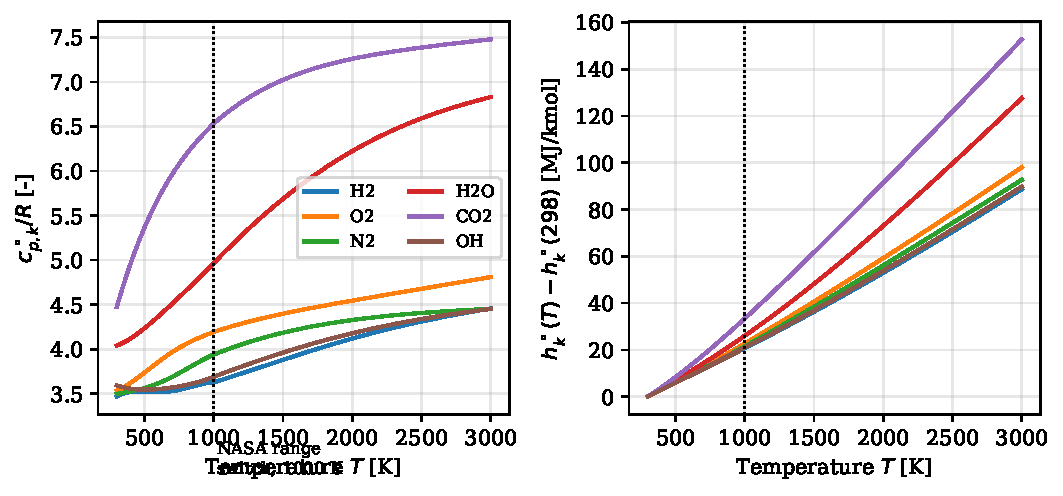
\includegraphics[width=\textwidth]{nasa_cp}
\caption{Left: $c_p/R$ from the NASA polynomials of GRI-Mech~3.0. Diatomics start near $3.5$
(translation + rotation) and grow as vibration switches on. \ce{H_2O} and \ce{CO_2} grow
more. Right: sensible enthalpy. The dotted line at \SI{1000}{\kelvin} is where the polynomial
ranges join; any kink there is a fitting artefact, not physics.}
\label{fig:nasa}
\end{figure}

\section{Mixture properties}

Ideal mixtures have no interaction energy, so mixture properties are simple averages of species
properties:
\begin{align}
  h&=\sum_kY_kh_k(T),\qquad c_p=\sum_kY_kc_{p,k}(T)\qquad\text{(per kg: mass-weighted)},\\
  \hat h&=\sum_kX_k\hat h_k(T)\qquad\text{(per kmol: mole-weighted)},\\
  s&=\sum_kY_k s_k(T,p,X_k)\qquad\text{(including the mixing term \eqref{eq:sk})}.
\end{align}

\begin{selfcheck}
\begin{enumerate}
  \item Why can the mixture enthalpy $h$ be negative? (Hint: \ce{H_2O} at room temperature.)
  \item A burnt-gas mixture has $h$ equal to that of the fresh gas, yet is at \SI{2300}{\kelvin}.
        Where did the ``chemical'' part of the enthalpy go?
  \item In \eqref{eq:hk}, which term changes when you preheat the reactants, and which when you
        change the fuel?
\end{enumerate}
\end{selfcheck}
